\section{\texorpdfstring{$k$}{k}-mer representation quality} \label{sec:K_mer_Representation}

Investigation on the anomalies resulted in two persistent clustering errors (\autoref{fig:PCA_Cluster_Knee_4} \textbf{\textsf{B}} and \textbf{\textsf{D}}). To evaluate if the method is suitable for the clustering of \gls{IAV} possible error sources are discussed.

% \begin{figure}[!hbt]
%     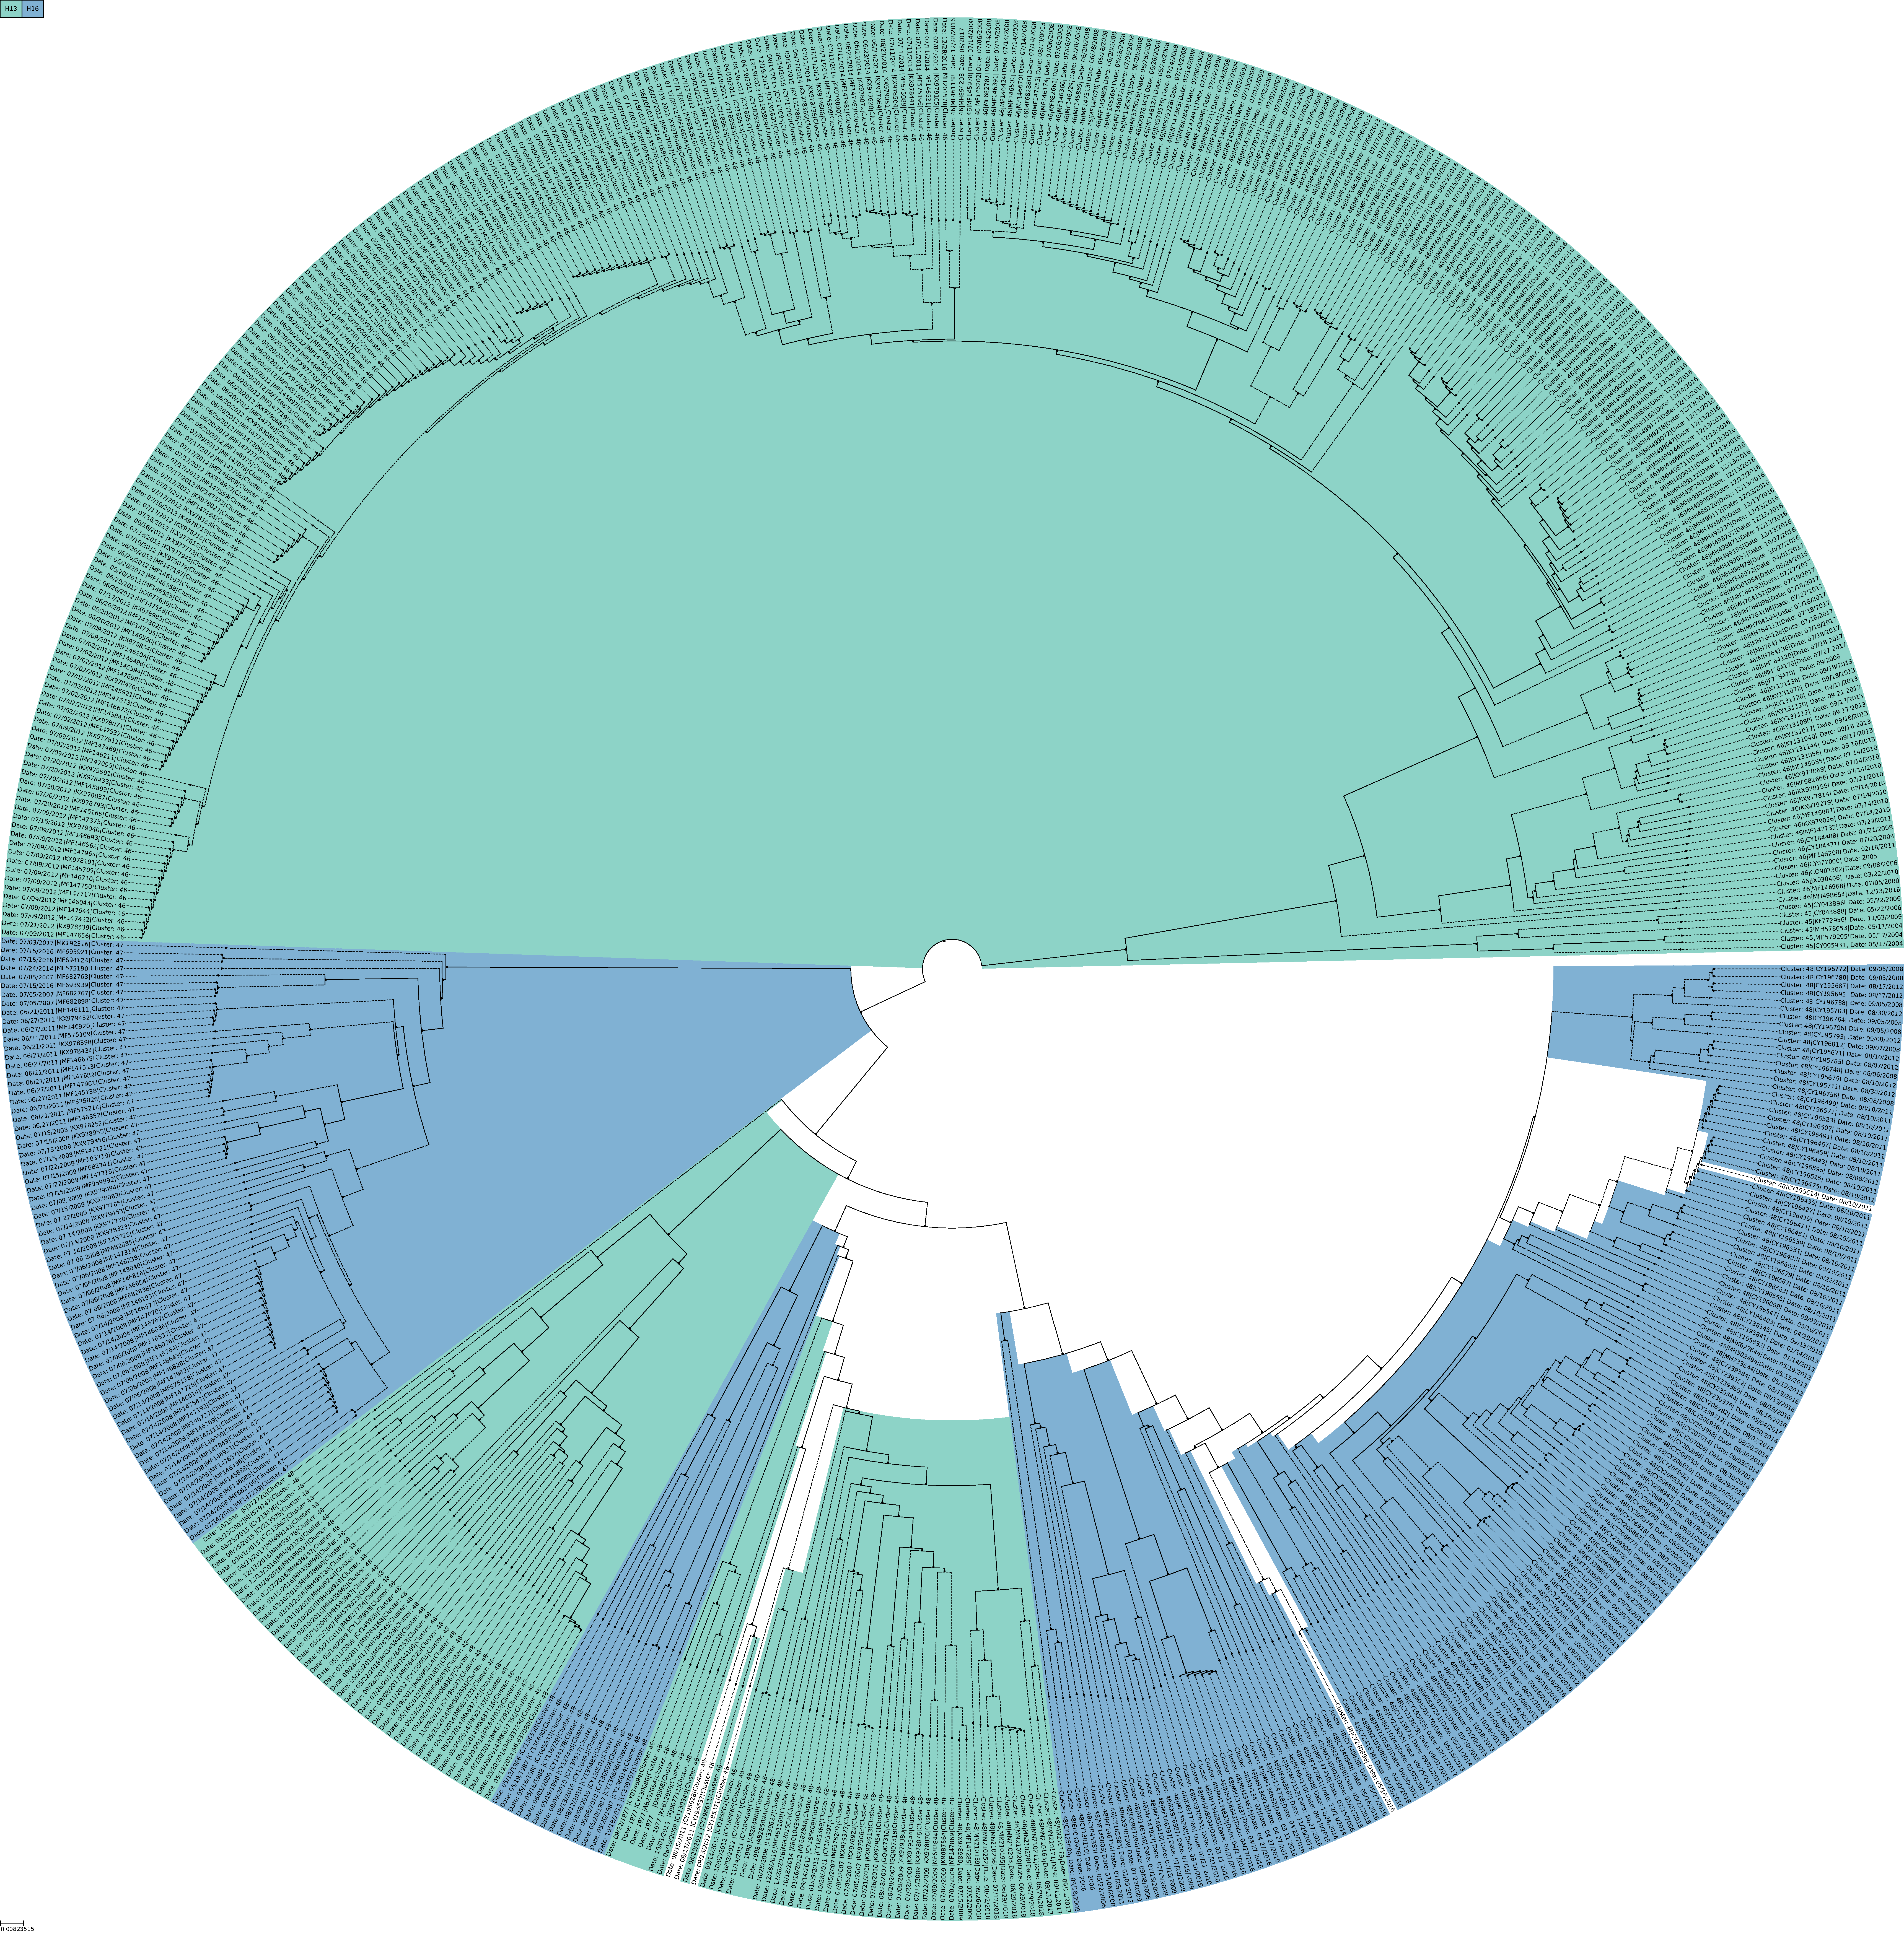
\includegraphics[width=\dimexpr\textwidth-2\fboxsep-2\fboxrule,fbox]{PCA/Clustertree_Segment_4_H_Knee_Zoom.pdf}
%     \caption[H13/H16 Simple Clustering Example with \texttt{PCA}]{\textbf{H13/H16 Simple Clustering Example with \texttt{PCA}.} .}
%     \label{fig:PCA_Clusteree_Knee_Zoom}
% \end{figure}

% \begin{figure}[!hbt]
%     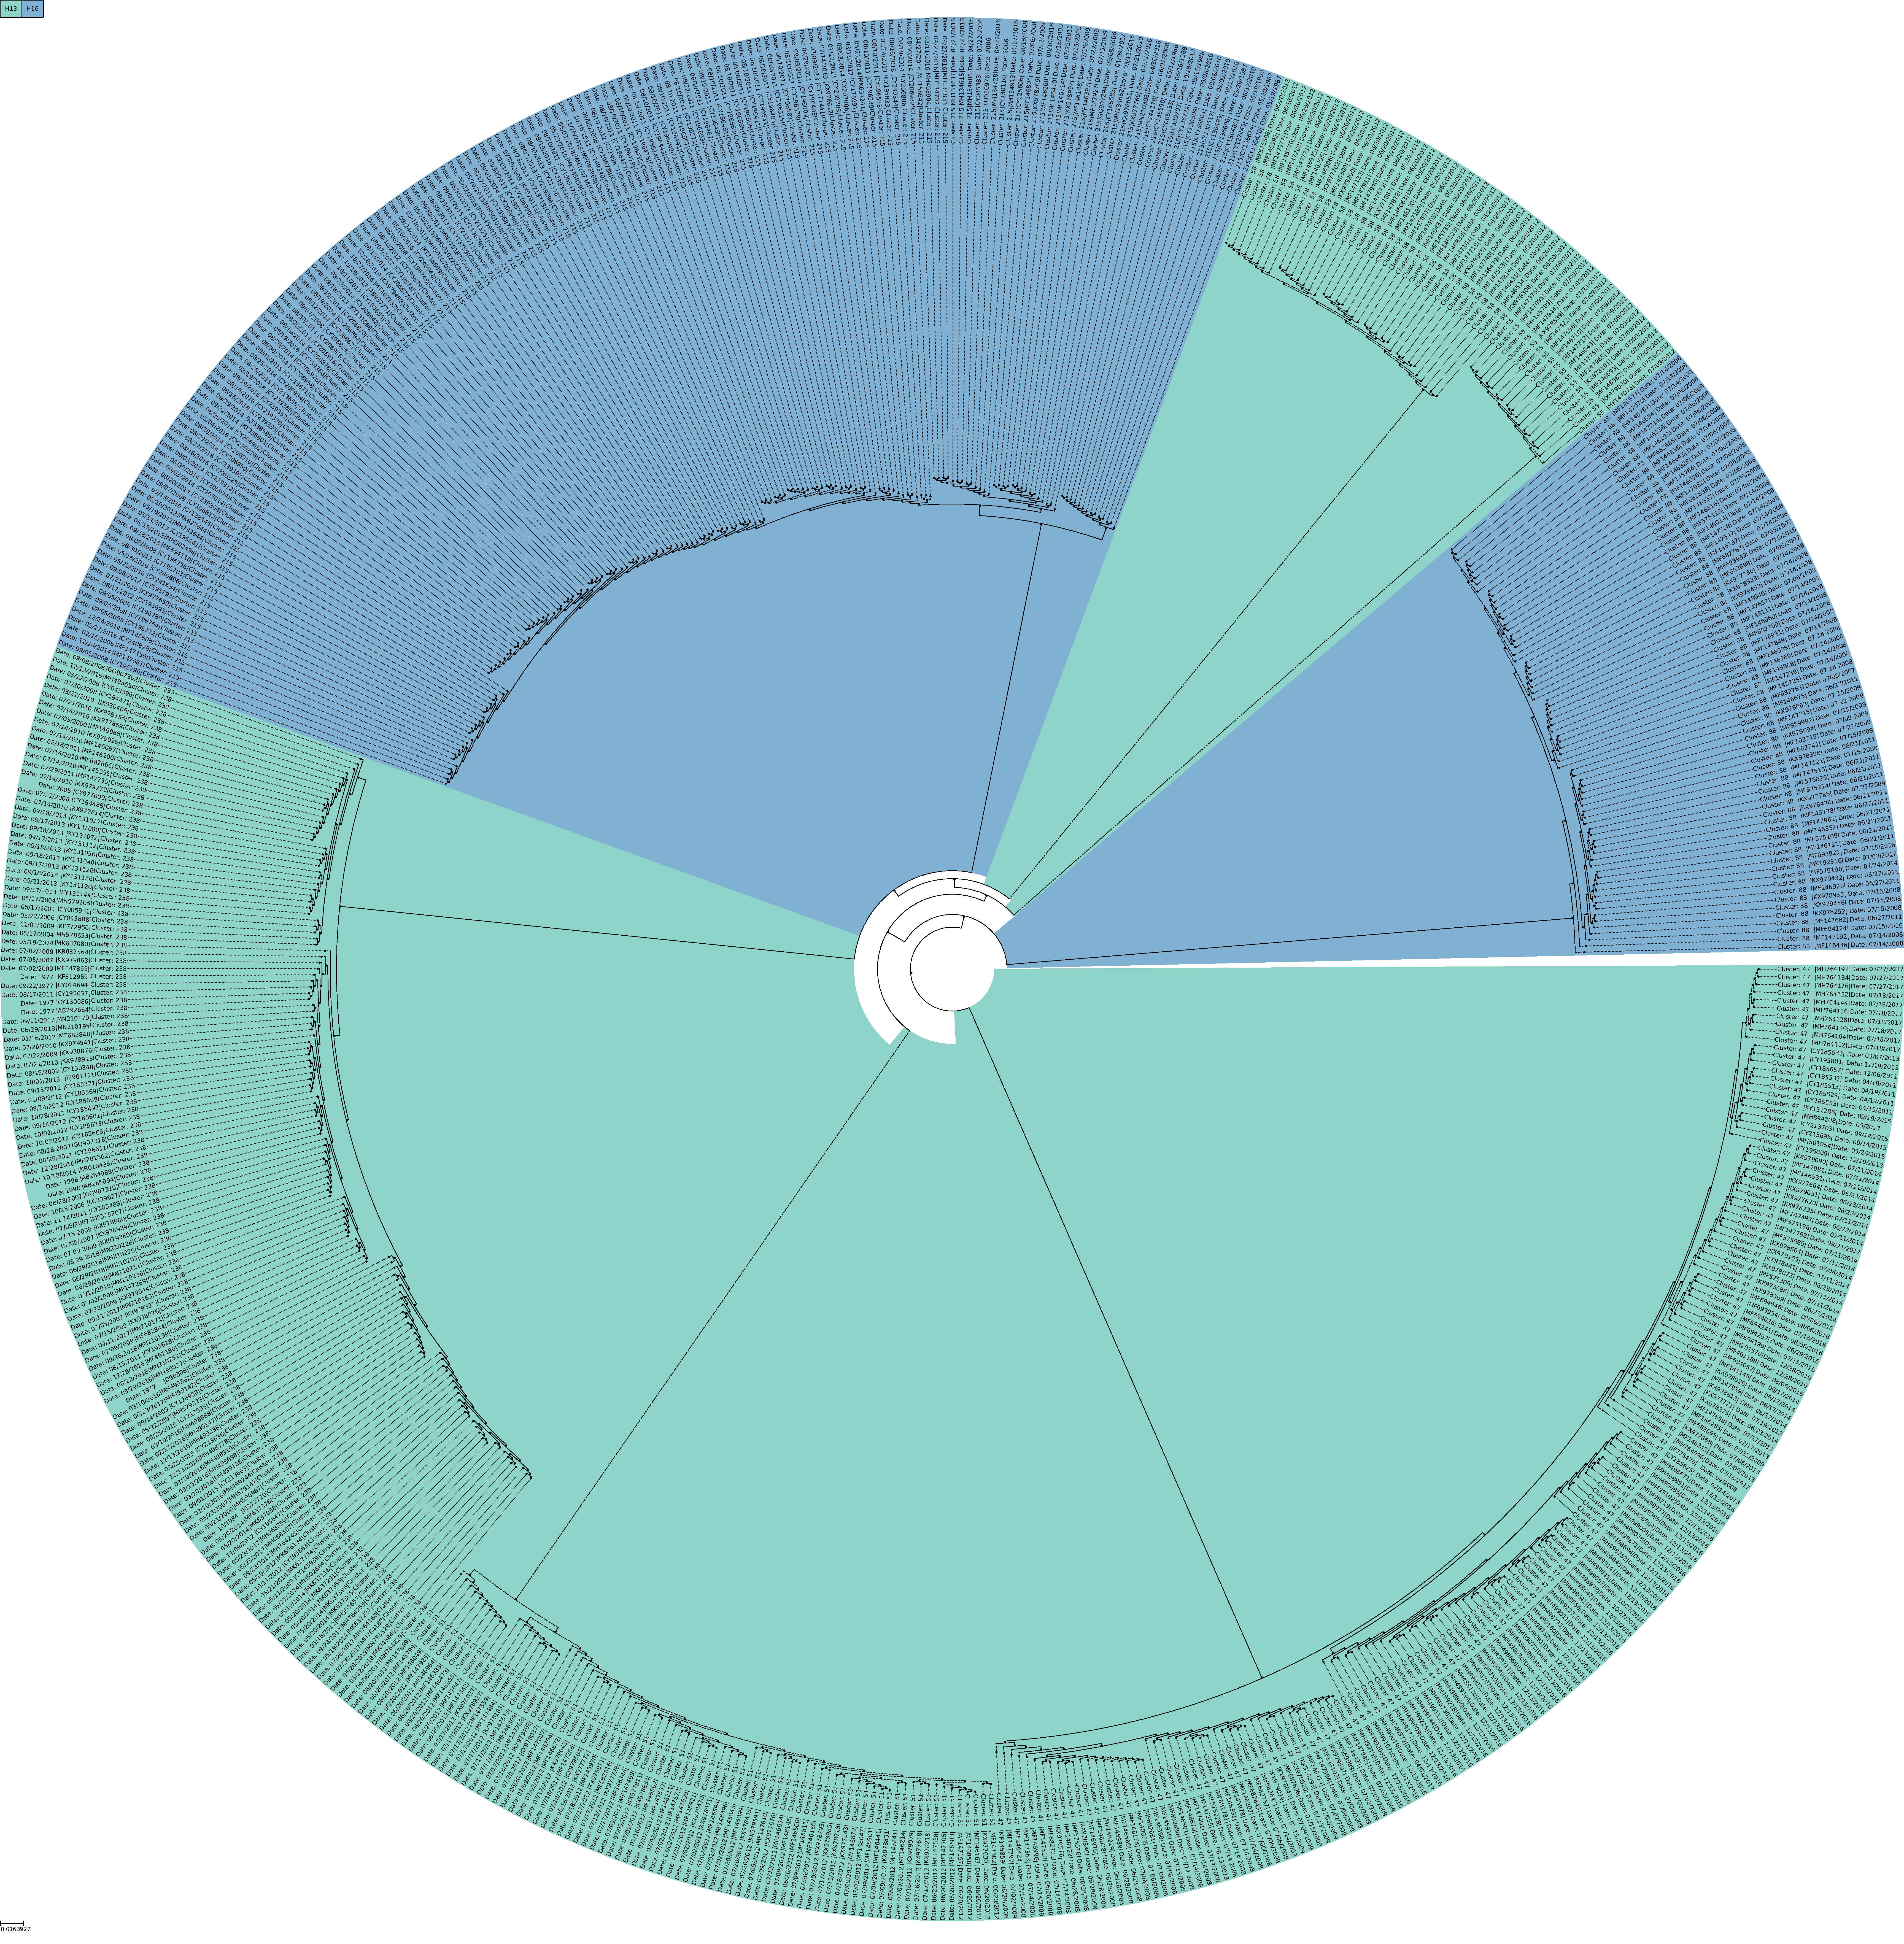
\includegraphics[width=\dimexpr\textwidth-2\fboxsep-2\fboxrule,fbox]{UMAP/Clustertree_Segment_4_H_Knee_Zoom.pdf}
%     \caption[H13/H16 Simple Clustering Example with \texttt{UMAP}]{\textbf{H13/H16 Simple Clustering Example with \texttt{UMAP}.} .}
%     \label{fig:UMAP_Clusteree_Knee_Zoom}
% \end{figure}

% \begin{figure}[!hbt]
%     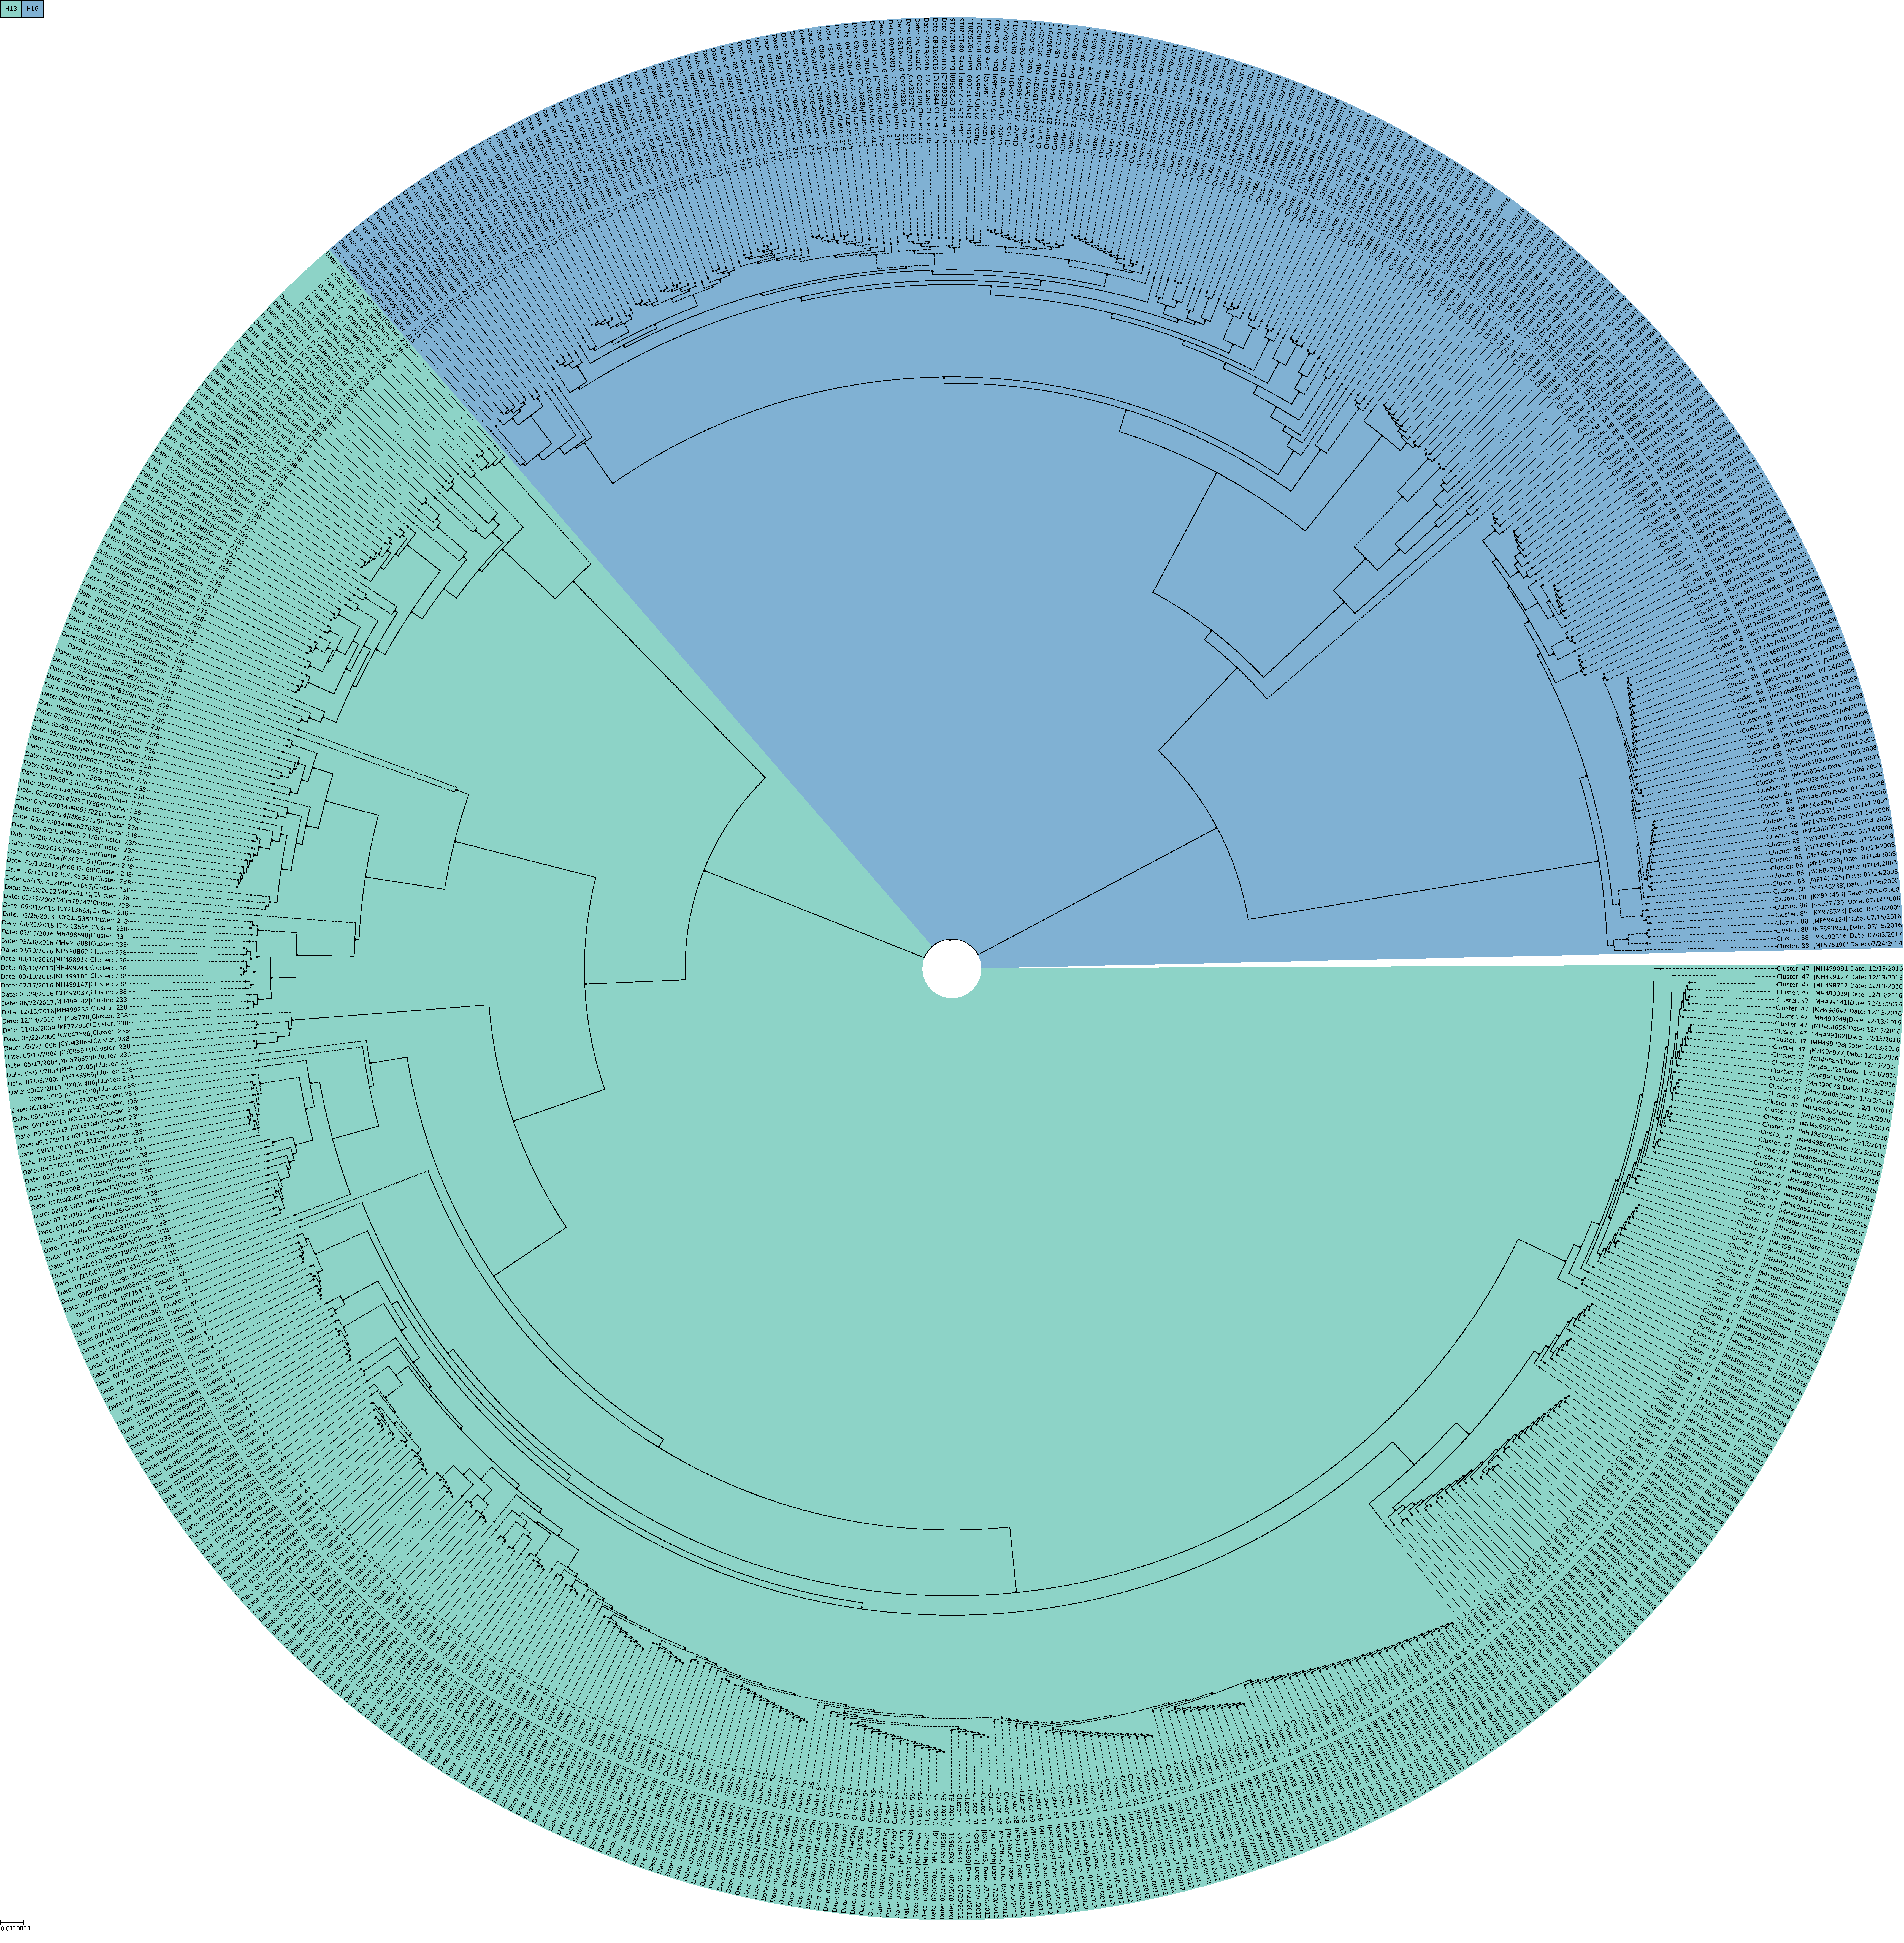
\includegraphics[width=\dimexpr\textwidth-2\fboxsep-2\fboxrule,fbox]{UMAP/Guidetree_Segment_4_H_Focus.pdf}
%     \caption[H13/H16 Simple Clustering Example with \Acrshort{MSA}]{\textbf{H13/H16 Simple Clustering Example with \Acrshort{MSA}.} .}
%     \label{fig:Guidetree_Focus}
% \end{figure}

\begin{figure}[!hbt]
    \centering
    \footnotesize
    \begin{tikzpicture}
        \node[anchor=south west,inner sep=0] (image) at (0,0) {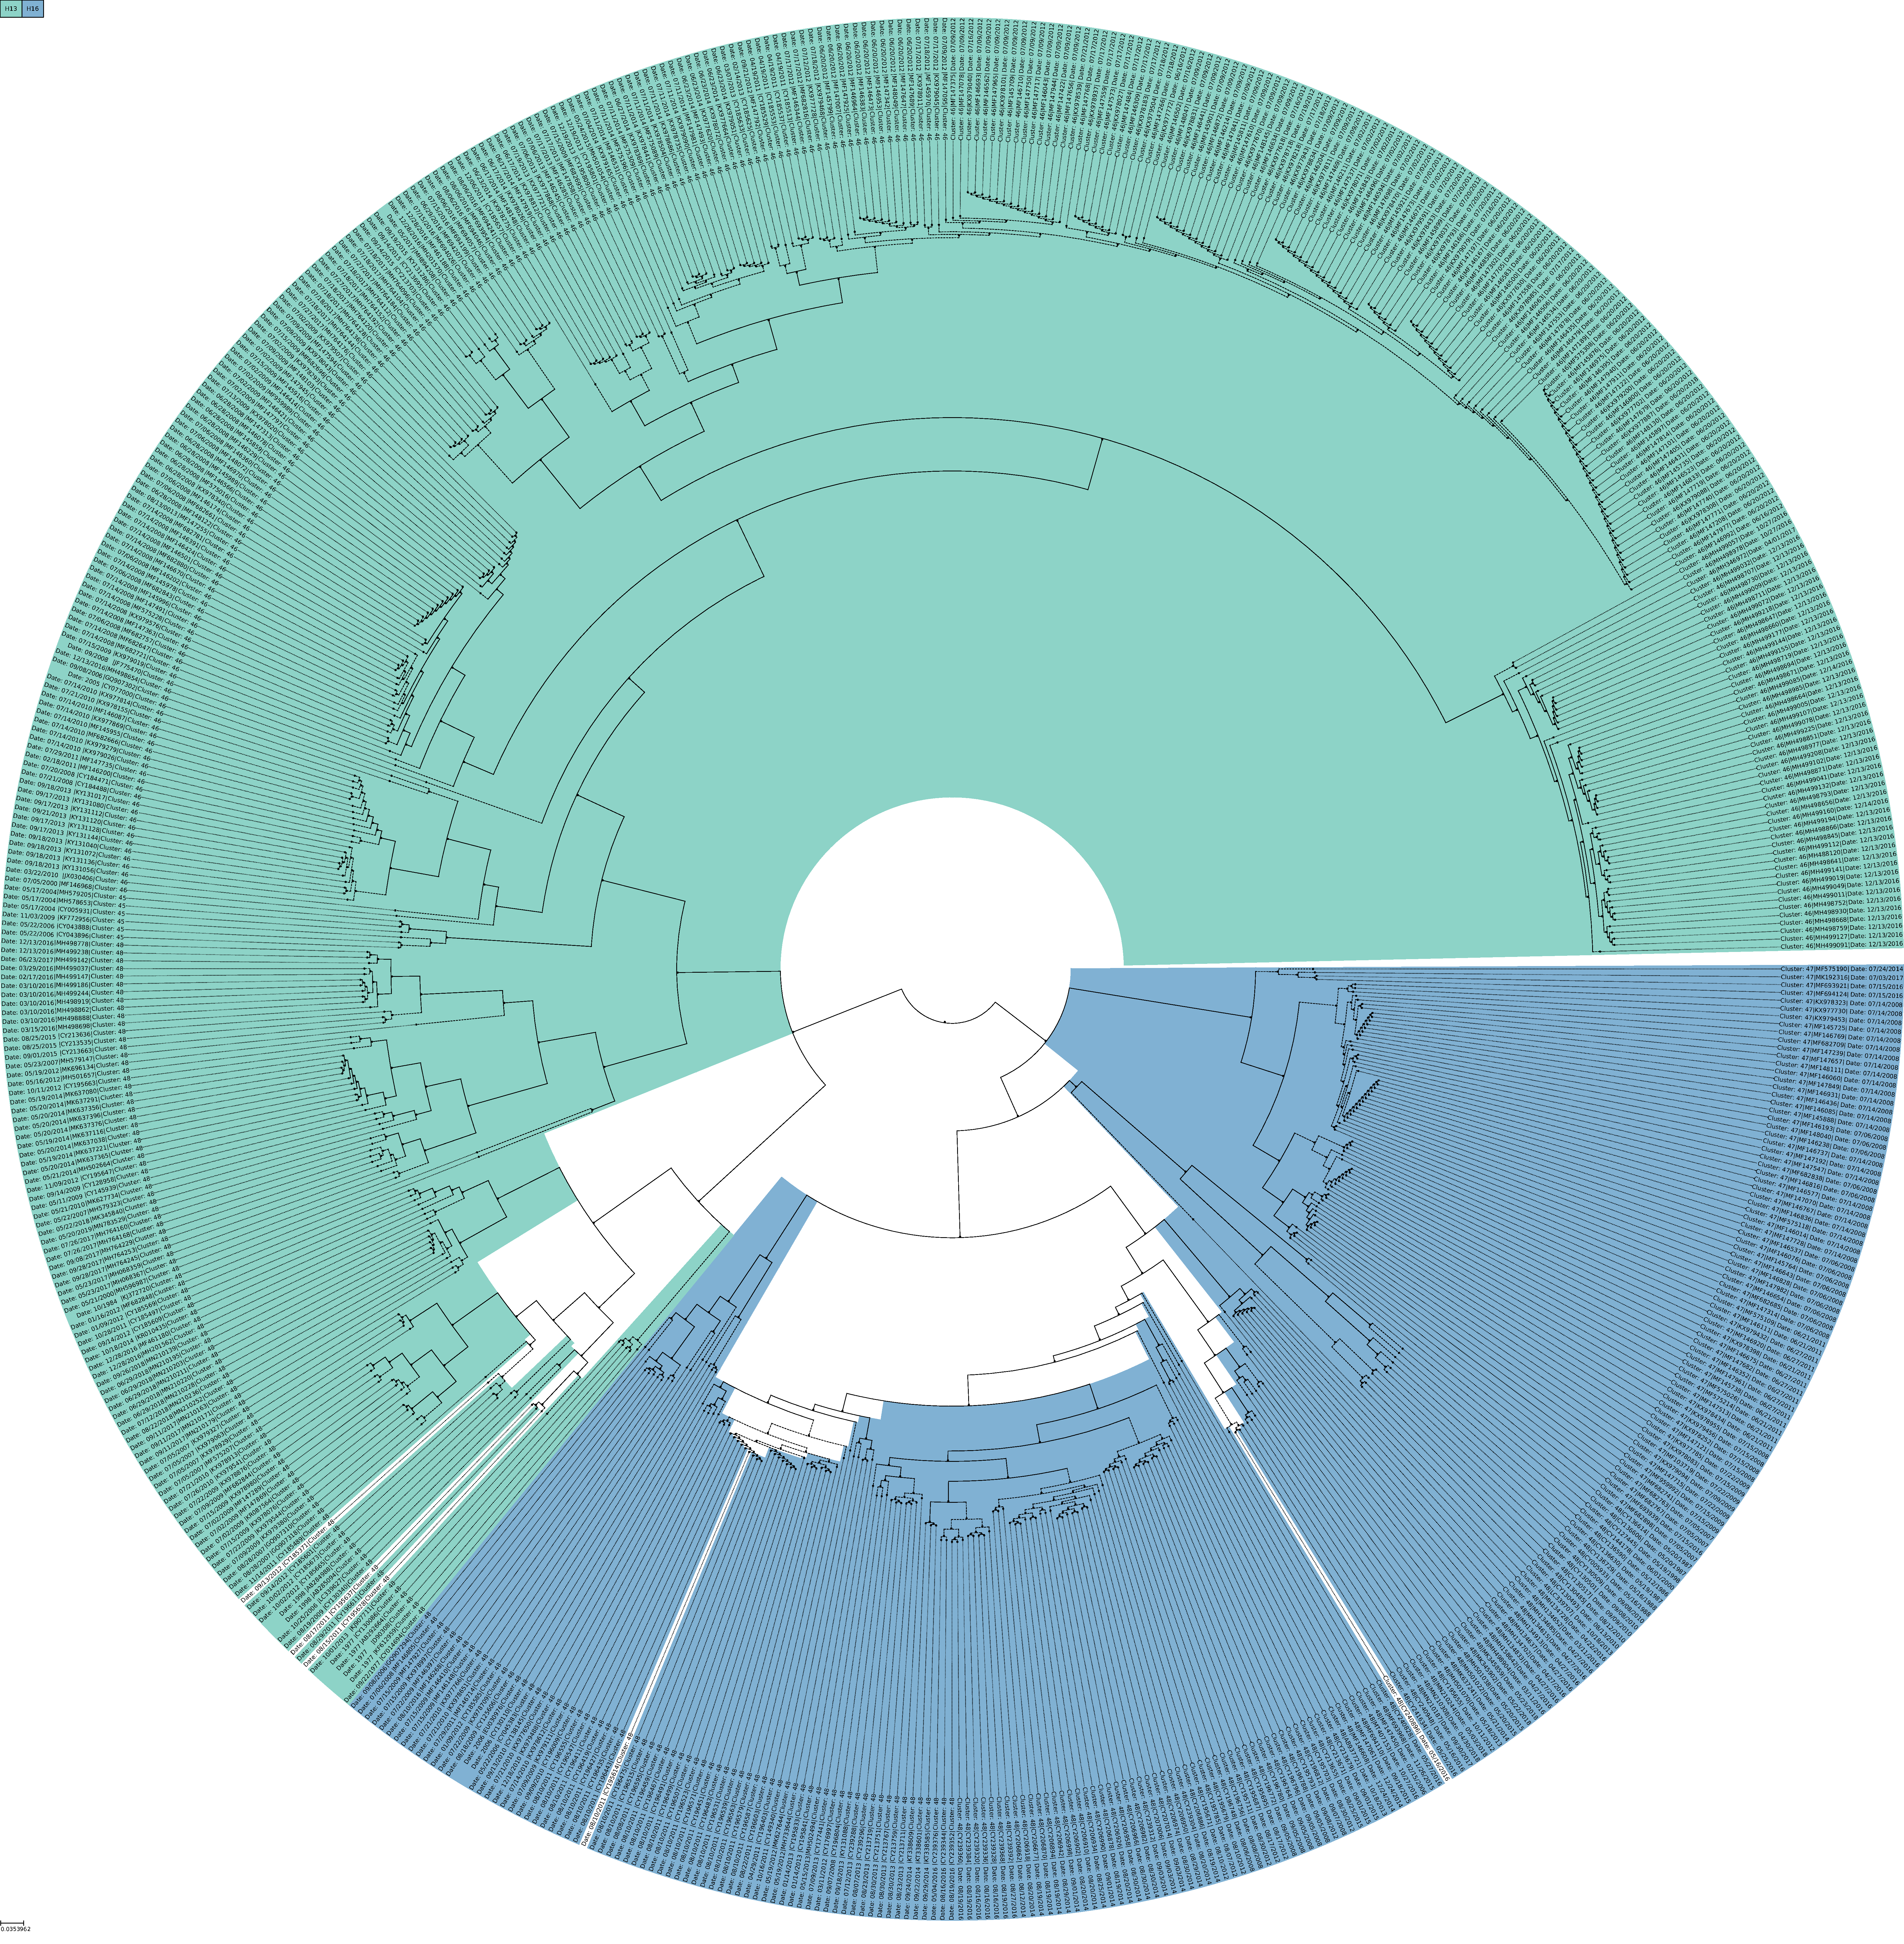
\includegraphics[width=\textwidth]{PCA/Precalculated_Segment_4_H_Cosine.pdf}};
        \begin{scope}[x={(image.south east)},y={(image.north west)}]
            %\draw[help lines,xstep=.1,ystep=.1] (0,0) grid (1,1);
            \draw[draw = none, fill = white] (0,1) rectangle (0.1,0.9);
            \draw[draw = none, fill = white] (0,0) rectangle (0.1,0.1);
            \draw[draw = black, thick, fill = black, fill opacity=0.0] (0.754,0.750) rectangle (0.999,0.505);
            \node at (0.754, 0.505) [fill=Red!80,thick,shape=circle,draw=black,inner sep=2pt] {\textbf{\textsf{C}}};
            %\draw[draw = black, thick, fill = black, fill opacity=0.2] (0.344, 0.603) rectangle (0.589,0.358);
            %\node at (0.344, 0.358) [fill=Red!80,thick,shape=circle,draw=black,inner sep=2pt] {\textbf{\textsf{A}}};
            \node at (0.425,0.525) [arrowstyle=1.0cm, arrowfillR, anchor=east, rotate=270] {\textbf{\textsf{A}}};
            \node at (0.55,0.525) [arrowstyle=1.0cm, arrowfillR, anchor=east, rotate=270] {\textbf{\textsf{B}}};
            %\draw[|-|] (0.975,0.5035) arc[start angle=0,end angle=170,radius=0.475, thick] node[midway,fill=Red!80,thick,shape=circle,draw=black,inner sep=2pt] {\textbf{\textsf{D}}};
            %\node at (0.5,0.505) [shape = circle,inner sep=140pt, fill = black] {};
            \node at (0.31,0.595) [arrowfillG, arrowstyle=1.0cm, anchor=east, rotate=315] {46};
            \node at (0.305,0.51) [arrowfillG, arrowstyle=1.0cm, anchor=east, rotate=45] {45};
            \node at (0.6,0.5) [arrowfillG, arrowstyle=1.0cm, anchor=east, rotate=225] {\rotatebox{180}{47}};
            \node at (0.35,0.455) [arrowfillG, arrowstyle=1.0cm, anchor=east, rotate=90] {48};
            \node at (0.425,0.42) [arrowfillG, arrowstyle=1.0cm, anchor=east, rotate=90] {48};
            \node at (0.54,0.435) [arrowfillG, arrowstyle=1.0cm, anchor=east, rotate=135] {\rotatebox{180}{48}};
        \end{scope}
    \end{tikzpicture}
    \caption[UPGMA tree of H13/H16 with cosine distance]{\textbf{UPGMA tree of H13/H16 with cosine distance.} Calculated cosine distance between the $k$-mer frequency vectors of sequences related to subtype H13 and H16 clusters in \autoref{fig:PCA_Clusteree_Knee_4} were used to build a \gls{UPGMA} tree. The same labeling of the previous tree was used to clarify the difference between H13 and H16 sequences. Unlabeled sequences are unclassified ones from the mixed cluster 48 and, thereby, not assigned to a single subtype. The numbers in the green arrows indicate the cluster number of the sub trees sequences in \autoref{fig:PCA_Clusteree_Knee_4}. The red arrows are used in the following to point to the trees division into H13 \textbf{\textsf{A}} and H16 \textbf{\textsf{B}}. \autoref{fig:focus} is a enlarged view on the highlighted square at \textbf{\textsf{C}}.}
    \label{fig:Precalculated_Cosine}
\end{figure}

By building a \gls{UPGMA} tree with cosine distance calculation on the non-reduced segment 4 $k$-mer frequency vectors with $4^7$ components of all the H13 and H16 sequences, the unbiased relation of sequences from these subtypes were analyzed (\autoref{fig:Precalc_Pipeline} workflow \textsf{\textbf{7}}). \gls{UPGMA} tree building was used on the alignment similar to \textcite{moss_identification_2011}. These calculations require high computation power and are only possible due to the small amount of segment 4 H13 and H16 sequences. Since no component reduction was performed in this case the fundamental use of $k$-mer frequencies could be validated or rejected. The tree was labeled in a similar way to the previous ones. Therefore, aiding the visualization, unclassified sequences were declared as a given subtype based on the clusters of \autoref{fig:PCA_Clusteree_Knee_4} again. The small amount of not labeled sequences in the \gls{UPGMA} tree are unclassified sequences, that also could not be assigned to a given subtype in the previous sections (not assigned sequences from mixed cluster 48). The labeling based on the clusters in \autoref{fig:PCA_Clusteree_Knee_4} was used to better visualize the separation and also reversely evaluate the labeling too. Outstanding labeling mistakes breaking the uniform separation would, thus, reject the assignment of not classified sequences, that was performed. All sequences in the \gls{UPGMA} tree were also annotated by their cluster number in \autoref{fig:PCA_Clusteree_Knee_4} to enable better comparison. The green arrows indicate sub trees in the \gls{UPGMA} tree containing the sequences assigned to a given cluster in the previous section. Sequences from cluster 46, 45 and 47 are contained in well separated sub trees, while the sequences of cluster 48 are spreaded over half the \gls{UPGMA} tree. This finding is in line with \autoref{fig:PCA_Cluster_Knee_4} error \textbf{\textsf{B}} and \autoref{fig:PCA_Guidetree_Centroid_4} indicating the existence of a clear separation of both subtypes even when a degree of similarity might exists.

\begin{figure}[!hbt]
    \centering
    %\begin{adjustbox}{minipage=\dimexpr\textwidth-2\fboxsep-2\fboxrule,fbox}
    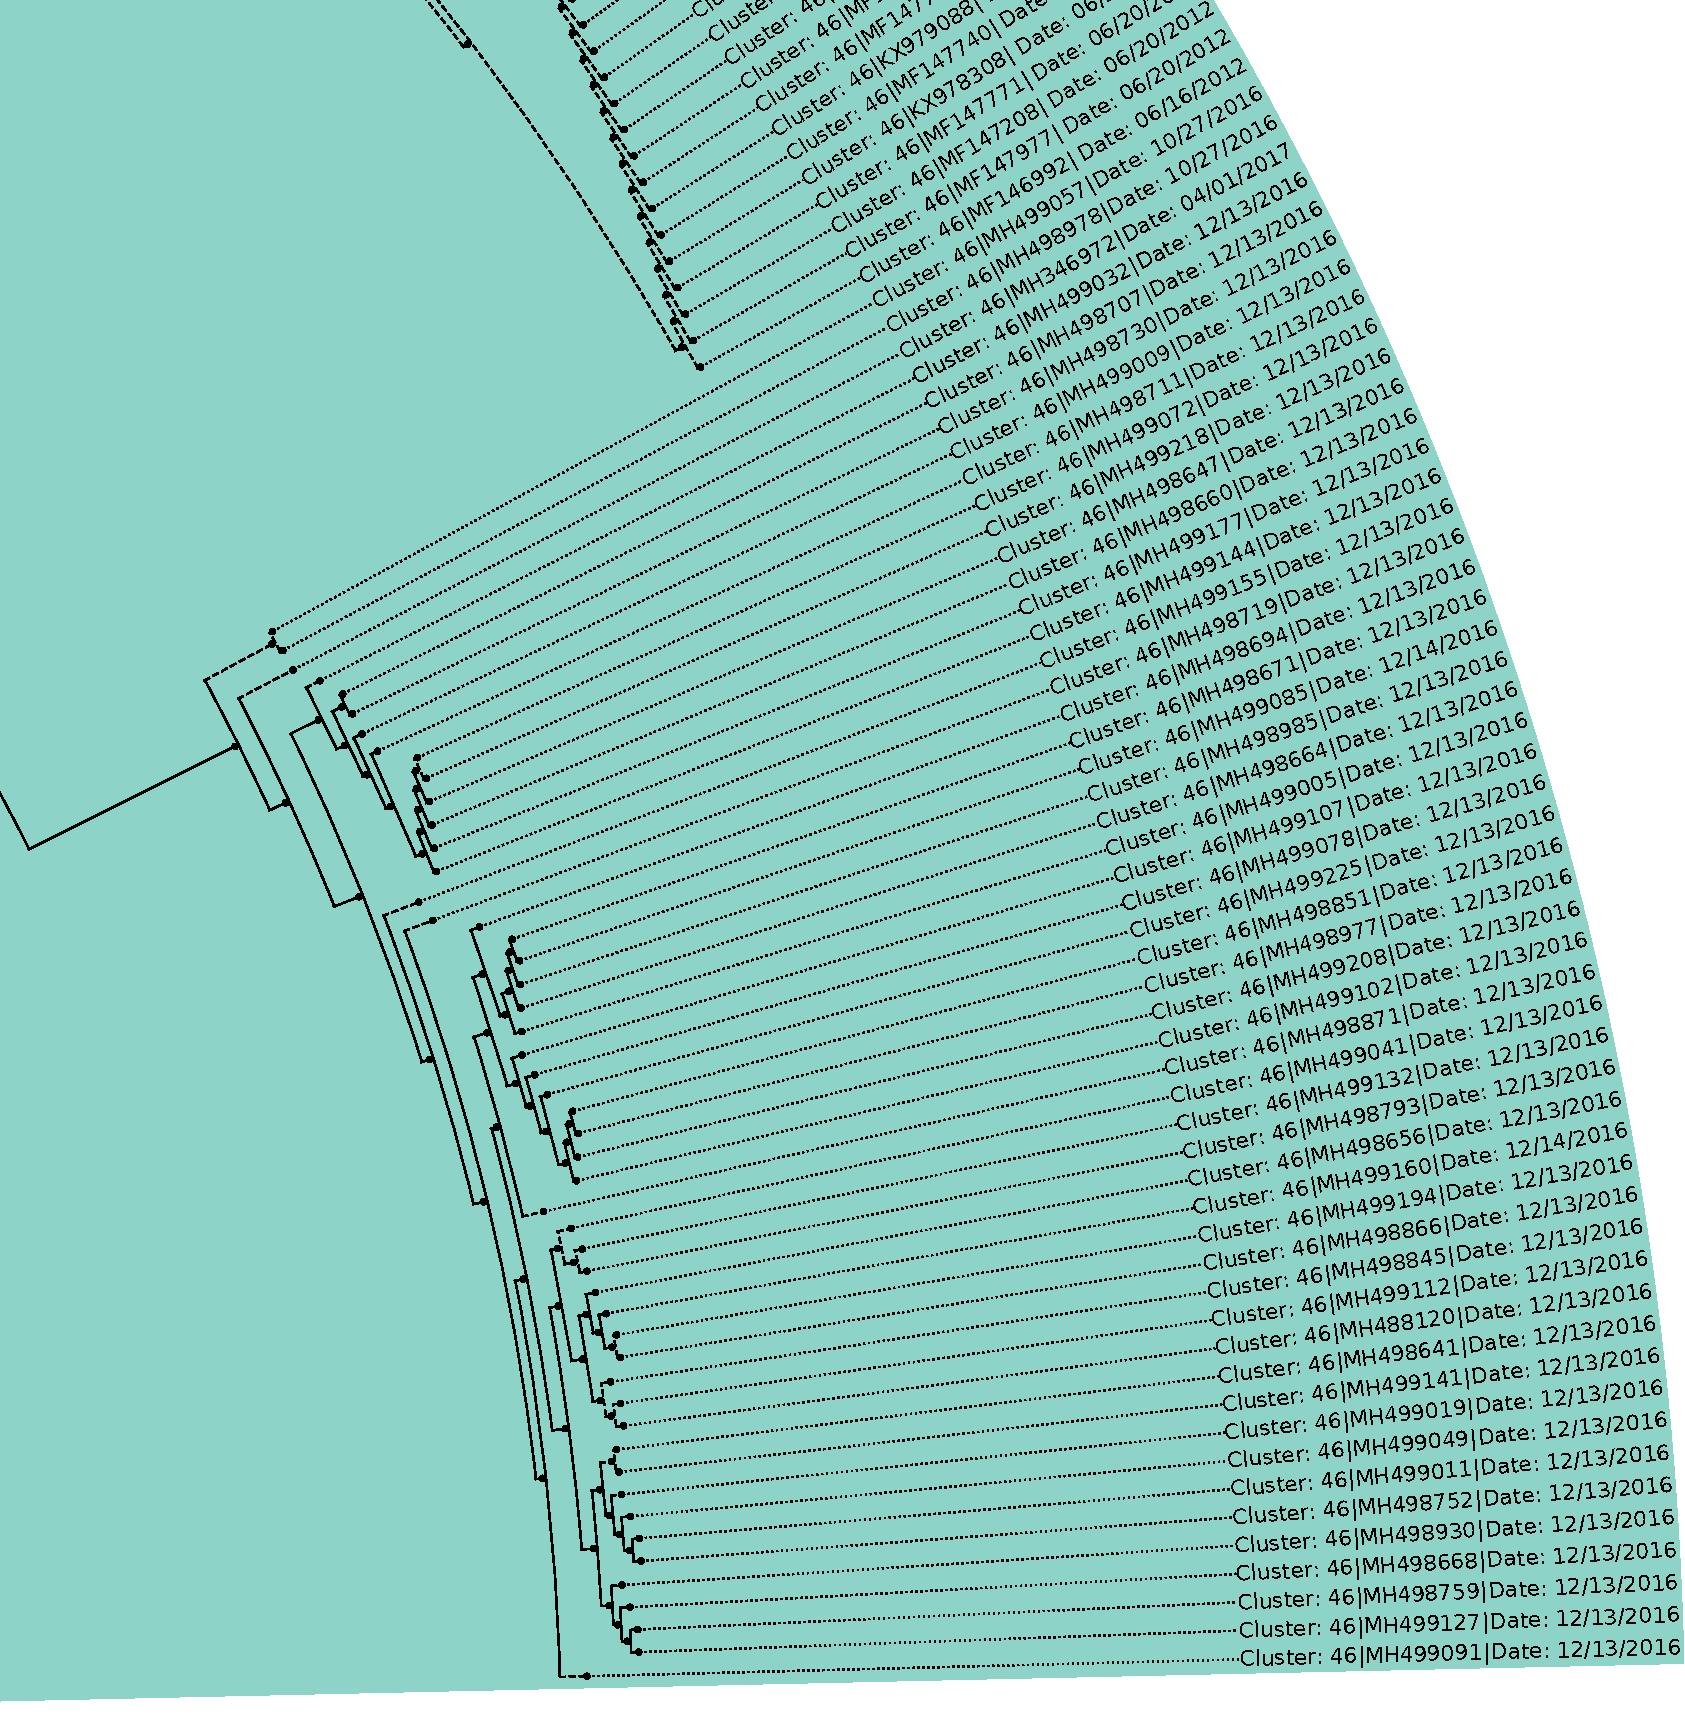
\includegraphics[width=\textwidth]{Graphics/identical.pdf}
    \caption[Relation of collection date and $k$-mer vector distance]{\textbf{Relation of collection date and $k$-mer vector distance.} Enlarged view of the by \textbf{\textsf{C}} highlighted square in \autoref{fig:Precalculated_Cosine}. The sequences were labeled according to their collection date to indicate the correlation of the close $k$-mer frequency vector distance in the tree with their sequences similarity. Labeling with the strain name could misleadingly point in a false direction, since the strain names indicate major difference while the sequences having very high similarity. Thereby the close distance of the vectors of sequences collected on the same date with high sequence similarity point to the precise representation by the $k$-mer frequency vectors.}
    \label{fig:focus}
\end{figure}

While both subtypes in \autoref{fig:Precalculated_Cosine} are completely separated directly after the trees root, there are also subsequent subdivisions for both subtypes directly after that. This early subdivision can point to the existence of more subtle variations with major difference to each other than the existing subtype classification reveals. In this case it appears as if at least two subgroups for H13 and at least two or three subgroups for H16 exist. The threshold is difficult to define, as no clustering was performed here. Thereby, this statement is based only on the early subdivision in the \gls{UPGMA} tree (\autoref{fig:Precalculated_Cosine} \textbf{\textsf{A}} and \textbf{\textsf{B}}). The exact separation from the root is in line with the centroid guide tree based on \gls{MSA} were both subtypes were completely separated too (\autoref{fig:PCA_Guidetree_Centroid_4}). Since this is also in line with the subtype classification, the $k$-mer frequency approach seemed to work as expected in this project. Furthermore, when focusing on a portion of the \gls{UPGMA} tree with very small distance in \autoref{fig:Precalculated_Cosine} \textbf{\textsf{C}}, the similar collection date of all these sequences (12/13/2016) stand out. The only sequences not from this collection date but, nevertheless, included in this sub tree are MH499057, MH498978, MH346972, MH499085, and MH499160. Two of the first three mentioned sequences are from the same collection date but some days prior to the rest, while the third was collected some days after the 12/13/2016. These three sequences are the last linked sequences in the sub tree with the highest distance in comparison to the rest and their collection date is nearly the same as for the rest. The other two sequences with different date MH499085 and MH499160 are in the middle of the sub tree but the collected just one day after the rest. This points in the direction that even small differences are noticed by the $k$-mer approach. The collection date was used as comparison here because many of the sequences in the sub tree have very different strain names but are almost or completely similar and, thereby, usage of the strain name instead could cause a misinterpretation. MH499085 of strain A/environment/Chile/C20369/2016 and MH498671 of strain A/white\_backed\_stilt/Chile/C20090/2016 differ by their strain names, as the virus was collected apparently completely different but the sequenced genomes are in fact 100\% the same. Around the tree in nearly every case similar collection dates have a small distance based on the $k$-mer frequency vectors, supporting the statement of the usability of $k$-mer frequencies for \gls{IAV} clustering. Same calculation for the precalculated \gls{UPGMA} tree was also repeated with euclidean distance (\autoref{fig:Precalculated_Euclid}) with the same result.

%frage is hier welche Methode die bessere representation ausstrahlt, sprich UMAP vgl. precalc ja/nein? dann PCA vgl precalc passt? ja/nein?